%        File: ans2012.tex
%     Created: Wednesday, January 25, 2012

\documentclass{anstrans}
%% To use the glossaries acronym package, you'll need to define any acronyms you intend to 
%% use. You can define acronyms with \newacronym{label}[acronym]{written out form}
%% To refer to them in the text use \gls{label}
\usepackage[acronym,toc]{glossaries}
\newacronym{MIT}{MIT}{the Massachusettes Institute of Technology}
\newacronym{UW}{UW}{University of Wisconsin}
\newacronym{US}{US}{United States}
\newacronym{SNF}{SNF}{spent nuclear fuel}
\newacronym{FEHM}{FEHM}{Finite Element Heat and Mass Transfer}
\newacronym{DOE}{DOE}{Department of Energy}
\newacronym{GENIUSv2}{GENIUS}{Global Evaluation of Nuclear Infrastructure Utilization Scenarios, Version 2}
\newacronym{CNERG}{CNERG}{Computational Nuclear Engineering Research Group}
\newacronym{GDSM}{GDSM}{Generic Disposal System Model}
\newacronym{GPAM}{GPAM}{Generic Performance Asessment Model}
\newacronym{FEPs}{FEPs}{Features, Events, and Processes}
\newacronym{EBS}{EBS}{Engineered Barrier System}
\newacronym{EDZ}{EDZ}{Excavation Disturbed Zone}
\newacronym{YMR}{YMR}{Yucca Mountain Repository Site}
\newacronym{EPA}{EPA}{Environmental Protection Agency}
\newacronym{PEI}{PEI}{Peak Environmental Impact}
\newacronym{VISION}{VISION}{the Verifiable Fuel Cycle Simulation Model}
\newacronym{NUWASTE}{NUWASTE}{Nuclear Waste Assessment System for Technical Evaluation}
\newacronym{NWTRB}{NWTRB}{Nuclear Waste Technical Review Board}
\newacronym{OCRWM}{OCRWM}{Office of Civillian Radioactive Waste Management}
\newacronym{UFD}{UFD}{Used Fuel Disposition}
\newacronym{DYMOND}{DYMOND}{Dynamic Model of Nuclear Development }
\newacronym{DANESS}{DANESS}{Dynamic Analysis of Nuclear Energy System Strategies}
\newacronym{CAFCA}{CAFCA}{ Code for Advanced Fuel Cycles Assessment }
\newacronym{ORION}{ORION}{O..}
\newacronym{NFCSim}{NFCSim}{Nuclear Fuel Cycle Simulator}
\newacronym{COSI}{COSI}{Commelini-Sicard}
\newacronym{FCT}{FCT}{Fuel Cycle Technology}
\newacronym{SWF}{SWF}{Separations and Waste Forms}
\newacronym{FCO}{FCO}{Fuel Cycle Options}
\newacronym{RDD}{RD\&D}{Research Development and Design}
\newacronym{WIPP}{WIPP}{Waste Isolation Pilot Plant}
\newacronym{ANDRA}{ANDRA}{Agence Nationale pour la gestion des D\'echets RAdioactifs, the French National Agency for Radioactive Waste Management}
\newacronym{TSM}{TSM}{Total System Model}
\newacronym{LANL}{LANL}{Los Alamos National Laboratory}
\newacronym{INL}{INL}{Idaho National Laboratory}
\newacronym{ANL}{ANL}{Argonne National Laboratory}
\newacronym{SNL}{SNL}{Sandia National Laboratory}
\newacronym{LBNL}{LBNL}{Lawrence Berkeley National Laboratory}
\newacronym{LLNL}{LLNL}{Lawrence Livermore National Laboratory}
\newacronym{NAGRA}{NAGRA}{National Cooperative for the Disposal of Radioactive Waste}
\newacronym{CUBIT}{CUBIT}{CUBIT Geometry and Mesh Generation Toolkit}
\newacronym{CSNF}{CSNF}{Commercial Spent Nuclear Fuel}
\newacronym{DSNF}{DSNF}{DOE Spent Nuclear Fuel}
\newacronym{HTGR}{HTGR}{High Temperature Gas Reactor}
\newacronym{TRISO}{TRISO}{Tristructural Isotropic}
\newacronym{MA}{MA}{Minor Actinide}
\newacronym{CEA}{CEA}{Commissariat a l'Energie Atomique et aux Energies Alternatives}
\newacronym{SKB}{SKB}{Svensk Karnbranslehantering AB}
\newacronym{SINDAG}{SINDA{\textbackslash}G}{Systems Improved Numerical Differencing Analyzer $\backslash$ Gaski}
%\newacronym{<++>}{<++>}{<++>}

\makeglossaries


%%%%%%%%%%%%%%%%%%%%%%%%%%%%%%%%%%%
\title{Numerical Calibration of an Analytical Generic Nuclear Repository Heat 
Transfer Model}
\author{Kathryn D.~Huff$^1$, Theodore H.~Bauer$^2$}

%% uncomment these next five only if using anstrans
\institute{$^1$Nuclear Engineering \& Engineering Physics Dept., University of 
Wisconsin, Madison, WI, 53706\\
$^2$Nuclear Engineering Division, Argonne National Laboratory, Argonne, IL, 
60439}
\email{$^1$khuff@cae.wisc.edu \& $^2$thbauer@anl.gov}
\usepackage{graphicx}
\usepackage{booktabs} % nice rules for tables
\usepackage{microtype} % if using PDF
\usepackage{bigints}
\newcommand{\units}[1] {\:\text{#1}}%
\newcommand{\SN}{S$_N$}%{S$_\text{N}$}%{$S_N$}%
\DeclareMathOperator{\erf}{erf}


\date{January 27, 2012}
%%%%%%%%%%%%%%%%%%%%%%%%%%%%%%%%%%%
\begin{document}
%%%%%%%%%%%%%%%%%%%%%%%%%%%%%%%%%%%%%%%%%%%%%%%%%%%%%%%%%%%%%%%%%%%%%%%%%%%%%%%%
\section{Introduction}

This work describes a benchmarking effort conducted to determine the accuracy of 
a new generic geology thermal repository model
relative to more traditional techniques and proposes a physically plausible auxillary thermal 
resistance component to improve their agreement.  

The analytic model to be calibrated was developed at 
\gls{LLNL}\cite{hardin_generic_2011,sutton_investigations_2011,greenberg_application_2012} 
and calulates the superposition of line and point source solutions representing 
a generic geology nuclear repository. It was benchmarked and calibrated against 
a numeric thermal model that utilizes a geometrically-explicit 
lumped-parameter modeling approach developed over several years at \gls{ANL} 
using the \gls{SINDAG} thermal modeling code 
\cite{gaski_sinda_1987,gaski_sindag_1987}.  Application of this approach to 
underground storage of heat generating nuclear waste streams within the proposed 
\gls{YMR} site has been widely reported \cite{wigeland_separations_2006}. 

The auxillary thermal resistance component improves the accuracy of the rapid 
analytic model by calibration against the numeric model.  Specificially, it 
improves estimations of the peak repository temperature as well as the timing of 
the peak temperature. 


%% RESULTS HERE %%

%%%%%%%%%%%%%%%%%%%%%%%%%%%%%%%%%%%%%%%%%%%%%%%%%%%%%%%%%%%%%%%%%%%%%%%%%%%%%%%%

%% The ANL model

\section{Background: Numerical SINDA{\textbackslash}G Model}

The numeric heat transport model created by the \gls{UFD} team at \gls{ANL} 
using the \gls{SINDAG} heat transport framework employs detailed finite-difference numeric  
models describing two distinct geometric arrangements: a single 
storage drift and an infinite array of identical, uniformly spaced  storage drifts.  
For a given waste stream, tunnel radius, and geologic parameters (i.e. thermal conductivity, density, and 
specific heat capacity), the model is able to compute the temperature field 
surrounding the tunnel wall and beyond.  

\subsection{Calculation Method}

The \gls{SINDAG} calculation engine uses a lumped parameter numeric model.
Originally created for optimal waste loading analysis of the \gls{YMR}, the 
model for an array of drifts is geometrically adjustable,  as illustrated in 
Figure \ref{fig:sindageom}. 

\begin{figure}[htbp!]
  \begin{center}
    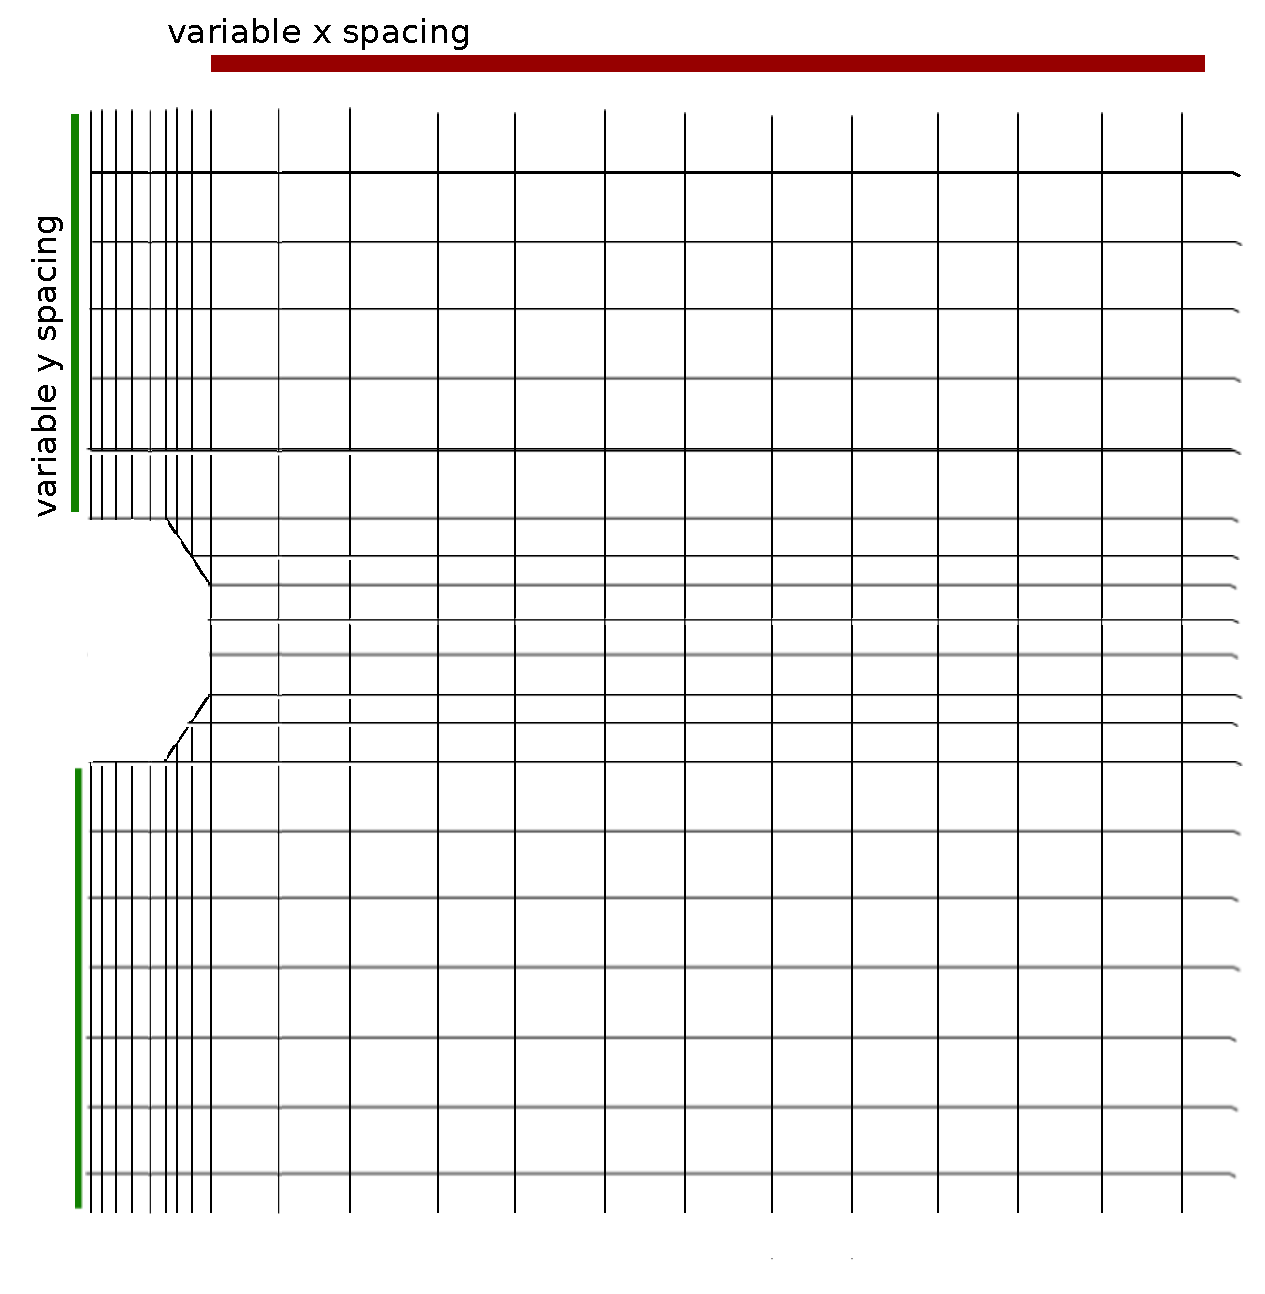
\includegraphics[width=0.4\textwidth]{./sindageom.eps}
  \end{center}
  \caption{The geometry of the 2D thermal model can be adjusted by altering 
  tunnel diameter, tunnel spacing, and the vertical distance below the surface.}
  \label{fig:sindageom}
\end{figure}

The \gls{SINDAG} lumped capacitance tool solves a thermal circuit, for which 
conducting nodes may be of four types corresponding to the four modes of heat 
transfer. Nodes are connected by conduction, convection, radiation, and mass 
flow heat transfer links. In the \gls{SINDAG} engine, these are represented by

\begin{align}
  R_{rad}  &= \frac{1}{\sigma F_{ij}A\left[ T_i + T_A + T_j + T_A 
  \right]\left[(T_i+T_A)^2+(T_j+T_A)^2\right]}\nonumber\\
  R_{cond} &= \frac{L}{K_{th} A}\mbox{, }R_{conv} = \frac{1}{h A}\mbox{, and 
  }R_{mf} = \frac{1}{\dot{m}c_p}
  \intertext{where}
  K_{th}&= ~~\mbox{thermal conductivity}[W\cdot m^{-1}\cdot K^{-1}]\nonumber\\
  A&= ~~\mbox{area} [m^2]\nonumber\\
  c_p&=~~\mbox{specific heat capacity} [J\cdot K^{-1}]\nonumber  \\
  h&= ~~\mbox{heat transfer coefficient}[W\cdot m^{-1} \cdot K^{-1}]\nonumber \\
  \dot{m}&= ~~\mbox{mass transfer rate}[kg\cdot s^{-1}]\nonumber \\
  T_i&= ~~\mbox{lump temperature} [^{\circ}C] \nonumber\\
  T_A&= ~~\mbox{absolute temperature} [^{\circ}C] \nonumber\\
  F_{ij}&= ~~\mbox{radiation interchange factor} [-] .\nonumber
\end{align}

Two \gls{SINDAG} model geometries have been used in this benchmark.  

\subsubsection{Single Drift}

In the single drift geometry, there is a distant fixed boundary condition and 
one waste tunnel is modeled with a continuous, cylindrical heat source of 
infinite length. The linear heat source in $[\frac{W}{m}]$ is modeled as if it 
is spread azimuthally over the surface of the drift tunnel. 

\subsubsection{Multiple Drift}

As llustrated in Figure \ref{fig:sindageom}, an infinite array of identical single-drift heat sources is modeled,
by assuming one-half of a storage tunnel with a reflective boundary condition at a vertical
plane midway between drifts. 

\section{Background: Analytical MathCAD Model}

The analytic model, created at \gls{LLNL} for the \gls{UFD} campaign seeks to 
inform heat limited waste capacity calculations for each lithology, for many 
waste package loading densities, and for many fuel cycle options 
\cite{hardin_generic_2011, sutton_investigations_2011, 
greenberg_application_2012}. It employs an analytic model from Carslaw and 
Jaeger and is implemented in MathCAD \cite{carslaw_conduction_1959, 
ptc_mathcad_2010}.  The integral solver in the MathCAD toolset is the primary 
calculation engine for the analytic MathCAD thermal model, which relies on 
superposition of integral solutions.  

\subsection{Calculation Method}

The model consists of two conceptual regions, an external region representing 
the host rock and an internal region representing the waste form, package, and 
buff \gls{EBS} within the disposal tunnel wall. The first region is taken to be  
a transient calculation unit.  Since the thermal mass of the \gls{EBS} is small 
in comparison to the thermal mass of the host rock, the internal region may be 
treated as quasi-steady state. The transient state of the temperature at the 
calculation radius is found with a convolution of the transient external 
solution with the steady state internal solution.  The process is then iterated 
with a one year resolution in order to arrive at a temperature evolution over 
the lifetime of the repository. 

\begin{figure}[h!]
  \begin{center}
    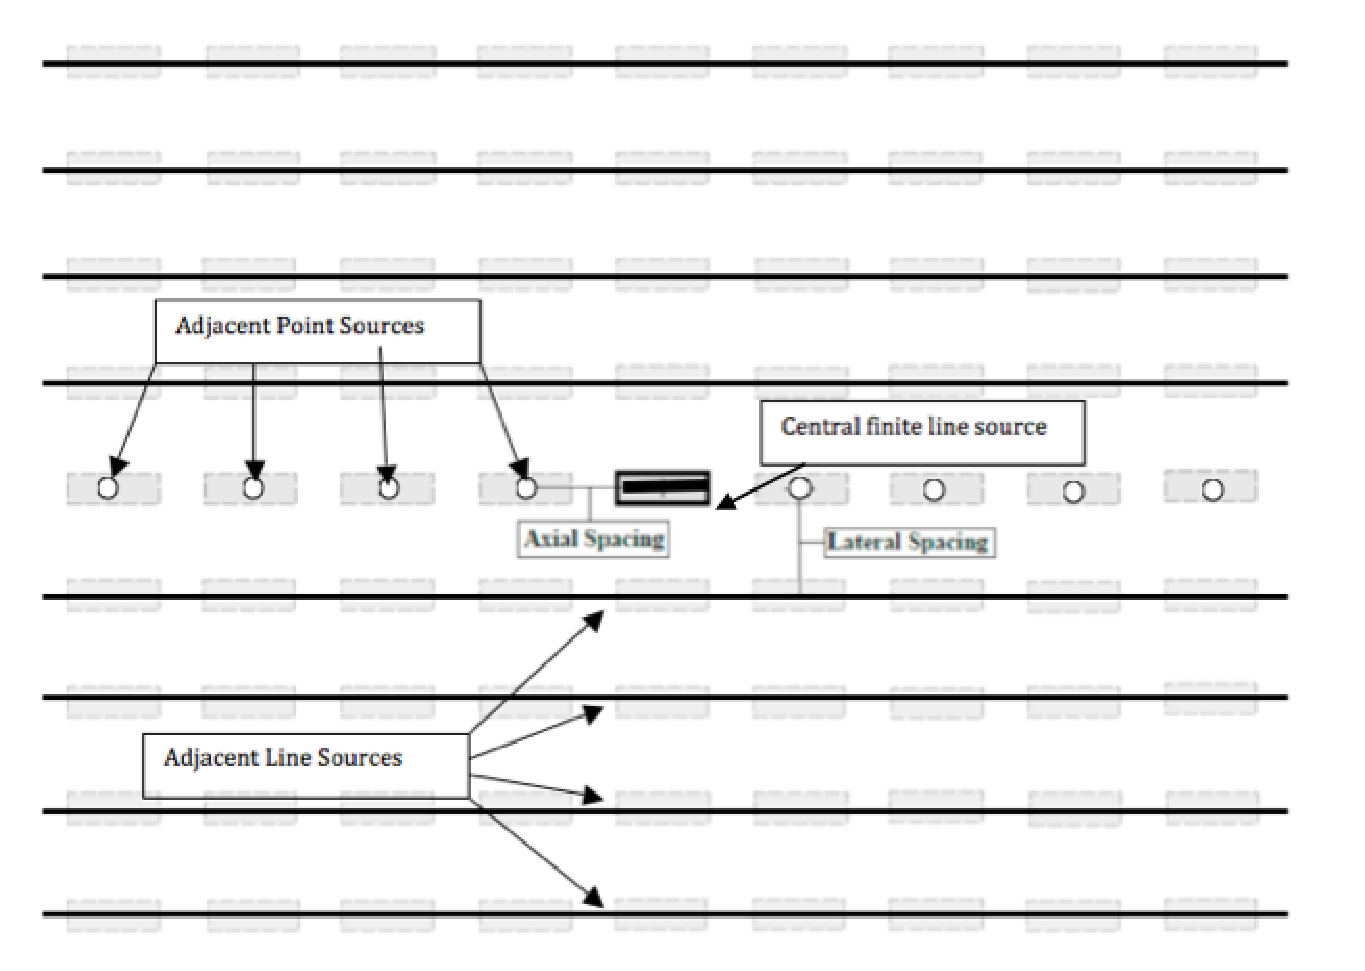
\includegraphics[width=0.5\textwidth]{llnlConcept.eps}
  \end{center}
  \caption{The central package is represented by a finite line source, adjacent 
  packages in the central drift are represented as points, and adjacent disposal 
  tunnes are represented as infinite lines.
  \cite{sutton_investigations_2011}.}
  \label{fig:llnl}
\end{figure}

The geometric layout of the analytic \gls{LLNL} model in Figure \ref{fig:llnl} 
shows  that the central package is represented by the finite line solution
\begin{align}
  T_{line}(t,x,y,z) &= \frac{1}{8\pi K_{th}} 
  \bigintsss_0^t\!\frac{q_L(t')}{t-t'}e^{ \frac{-\left(x^2 + z^2\right)}{4\alpha 
  (t-t')} }\nonumber\\ &\cdot\left[ \erf{\left[ \frac{1}{2} \frac{\left( y + 
  \frac{L}{2} \right)}{\sqrt{\alpha(t-t')}}  \right]} - \erf{\left[ \frac{1}{2} 
  \frac{\left( y - \frac{L}{2} \right)}{\sqrt{\alpha(t-t')}}  \right]} 
  \right]\,\mathrm{dt'},
  \label{line}
  \intertext{adjacent packages within the central tunnel are represented by the 
  point source solution }
  T_{point}(t,r) &= 
  \frac{1}{8K_{th}\sqrt{\alpha}\pi^{\frac{3}{2}}}\bigintsss_0^{-t}\!\frac{q(t')}{(t-t')^{\frac{3}{2}}}e^{\frac{-r^2}{4\alpha(t-t')}}\,\mathrm{dt'},
  \label{point}
  \intertext{and adjacent disposal tunnels are represented by infinite line 
  source solutions}
  T_{\infty line}(t,x,z) &= \frac{1}{4\pi K_{th}} 
  \bigintsss_0^t\!\frac{q_L(t')}{t-t'}e^{ \frac{-\left(x^2 + z^2\right)}{4\alpha 
  (t-t')} }
  \intertext{in infinite homogeneous media, where}
  \label{infline}
  \alpha &= ~~\mbox{thermal diffusivity } [m^2\cdot s^{-1}]\nonumber\\
  q(t) &= ~~\mbox{point heat source} [W]\nonumber\\
  \intertext{and}
  q_L(t) &= ~~\mbox{linear heat source} [W\cdot m^{-1}]\nonumber
\end{align}
Superimposed point and line source solutions allow for a notion of the 
repository layout to be modeled in the host rock.

%%%%%%%%%%%%%%%%%%%%%%%%%%%%%%%%%%%%%%%%%%%%%%%%%%%%%%%%%%%%%%%%%%%%%%%%%%%%%%%%
\section{Results of Comparative Analyses}

\subsection{Benchmarking}

Benchmarking results shown in Tables \ref{tab:benchMulti} and 
\ref{tab:benchSingle} below  effort between the analytic \gls{LLNL}
model and the numeric \gls{SINDAG} \gls{ANL} models illustrate the degree of agreement 
between analytic and numeric models. In particular, the analytic model would seem 
well-suited for purposes of rapid evaluation of generic geologic repository configurations. 

Specifically, for the single drift geometry benchmark, the 
analytic model gave peak temperatures for all cases run which agreed with the 
numeric model within $4^{\circ}C$ and, for calculation radii less than 5 meters, 
consistently reported peak temperature timing within 11 years of the \gls{ANL} 
numeric model. For the multiple drift case, in which the numeric model 
approximated an infinite array of drifts and the analytic approach modeled 101, 
the differences between models were slightly greater. The benchmarking cases run 
in this validation effort are listed in Table \ref{tab:benchSingle} and for the 
simplified single drift and in Table \ref{tab:benchMulti} for the multiple drift 
case.

In light of the magnitude of uncertainties involved in generically 
modeling a non-site-specific geologic repository, this sufficiently validated 
the analytic \gls{LLNL} model with respect to its goals.

The benchmark revealed a notable discrepancy between the two models, 
however. The time of peak heat arrived consistently sooner and the value of the 
peak temperature was consistently lower in the homogeneous medium analytic
model than in the numeric model. 

\begin{table}
  \centering
  \footnotesize{
  \begin{tabular}{|l|l|l|l|l|l|l|}
    \multicolumn{7}{c}{\textbf{Benchmarking Results for Single Drift 
    Scenario}}\\
    \hline
    & \multicolumn{6}{|c|}{Peak Temperature Discrepancy}\\ 
    & \multicolumn{6}{|c|}{$T_{peak,num}-T_{peak,an}$ $[^{\circ}C]$} \\
    \hline
    Material & \multicolumn{3}{|c|}{Clay} & \multicolumn{3}{|c|}{Salt}\\ & 
    \multicolumn{3}{|c|}{$K_{th}=2.5$} & \multicolumn{3}{|c|}{$K_{th}=4.2$}\\ & 
    \multicolumn{3}{|c|}{$\alpha=1.13\times10^{-6}$} & 
    \multicolumn{3}{|c|}{$\alpha=2.07\times10^{-6}$}\\ 
    \hline
    Years Cooling  & 10     & 25      & 50      & 10     & 25     & 50\\
    \hline
     R=0.35m  & 3.0   & 2.3     & 1.6    & 2.0   & 1.7   & 1.2\\
     R=0.69m  & 3.1   & 2.4    & 1.6    & 2.2    & 1.8   & 1.3\\
     R=3.46m  & 2.1   & 1.9    & 1.5    & 2.2   & 1.7    & 1.3\\
     R=7.04m  & 3.1   & 2.4     & 1.8    & 2.5   & 2.1   & 2.2\\
     R=14.32m & 3.6   & 2.9    & 2.1    & 2.8   & 2.6   & 3.7\\
    \hline
    & \multicolumn{6}{|c|}{Peak Heat Timing Discrepancy}\\ 
    & \multicolumn{6}{|c|}{ $t_{peak,num}-t_{peak,an}$ [yr]} \\
    \hline
    Material & \multicolumn{3}{|c|}{Clay} & \multicolumn{3}{|c|}{Salt}\\ & 
    \multicolumn{3}{|c|}{$K_{th}=2.5$} & \multicolumn{3}{|c|}{$K_{th}=4.2$}\\ & 
    \multicolumn{3}{|c|}{$\alpha=1.13\times10^{-6}$} & 
    \multicolumn{3}{|c|}{$\alpha=2.07\times10^{-6}$}\\ \hline
    Years Cooling  & 10     & 25      & 50      & 10     & 25     & 50\\
    \hline
     R=0.35m  & 1    & 1       & 1   & 1      & 1      & 3\\
     R=0.69m  & 2    & 2       & 1    & 2      & 3      & 4\\
     R=3.46m  & 9    & 7       & 6    & 4      & 2      & 11\\
     R=7.04m  & 4    & 13      & 10    & 11     & 10     & 288\\
     R=14.32m & 16   & 14      & 21   & 17     & 285    & 282\\
    \hline
  \end{tabular}
  \caption{Benchmarking in the single drift case showed that the peak heat was 
  calculated to be lower and arrived consistently sooner in the analytic (an) 
  model than in the numeric (num) model. 
  }
  \label{tab:benchSingle}
  }
\end{table}

\begin{table}
  \centering
  \footnotesize{
  \begin{tabular}{|l|l|l|l|}
    \multicolumn{4}{c}{\textbf{Benchmarking Results for 101 Drift Scenario}}\\
    \hline
    Material & \multicolumn{3}{|c|}{Clay} \\
    & \multicolumn{3}{|c|}{$K_{th}=2.5$}\\ 
    & \multicolumn{3}{|c|}{$\alpha=1.13\times10^{-6}$}  \\
    \hline
    & \multicolumn{3}{|c|}{Peak Temperature Discrepancy} \\
    & \multicolumn{3}{|c|}{$T_{peak,num}-T_{peak,an}$ $[^{\circ}C]$} \\
    \hline
    Years Cooling  & 10  & 25 & 50 \\
    \hline
    R=0.35m   & 7 & 4.6 & 2.1 \\
    \hline
    &\multicolumn{3}{|c|}{Peak Heat Timing Discrepancy}\\
    &\multicolumn{3}{|c|}{ $t_{peak,num}-t_{peak,an}$ [yr]} \\
    \hline
    R=0.35m       & -13.5   & 2   & -6  \\
    \hline
  \end{tabular}
  \caption{Benchmarking in the multiple drift case showed that the peak heat was 
  calculated to be consistently lower in the analytic (an) model and deviated further
  from the numeric (num)  model than did the single drift case.
  }
  \label{tab:benchMulti}
  }
\end{table}


\subsection{Calibration}

The goal of the calibration effort is accurate estimation of temperature fields in 
geologic repositories both across large expanses of host rock over long time 
spans using the analytic model and locally, over much shorter time spans within the 
engineered barrier systems using the numeric model.  Physically, it would be expected 
that the analytic line source model provides accurate temperatures across large spans
of a repository over large spans of time in regions far enough from storage units that 
heat generated in the repository would be accurately described as line sources. It is also
possible the model's accuracy in the vicinity of tunnel walls or waste package 
configurations can be improved by "calibration" against the SINDAG models discussed can  
be expected to accurately model temperatures close in to engineered storage units 
and in shorter time frames.

It is assumed that \gls{EBS} components within the disposal tunnel are only a 
small volume fraction of the rock. Due to the high heat conductivity materials 
in the \gls{EBS} it can be assumed that in reality, the temperature field in the
\gls{EBS} responds to changes in the waste package decay heat more rapidly than 
the field in the surrounding host rock. This behavior is not taken into account
in the analytic model, but is explicitly accounted for in the numeric model. The following
simple empirical expression is plausibly added to the analytic model to more accurately
estimate temperatures at locations within storage drifts. 

The difference in temperature due to the instantaneous transient response in the  
tunnel is here modeled as $\Delta T$, 

\begin{align}
  \Delta T(t) &= T_{numeric}(r_{t}) - T_{analytic}(\frac{D_d}{2})\\ 
  \Delta T(t) &= C q_L(t) 
  \frac{1}{K_{th}}\frac{1}{D_d}\\
  \intertext{where}
  D_{d} &= \mbox{Distance between drifts} [m]\nonumber\\
  r_{t} &= \mbox{Tunnel wall radius, calculation radius} [m]\nonumber
  \intertext{and}
  C &= \mbox{A coefficient derived from fitting}[m].\nonumber
  \label{deltat}
\end{align}

This allows the capacitive behavior of the model to remain entirely in the 
analytic model, and embeds the resistive behavior in a purely algebraic 
calibration. The calibration is valid for all repository configurations which 
share a tunnel diameter, tunnel spacing, and host rock material.

\begin{figure}[h!]
  \centering
    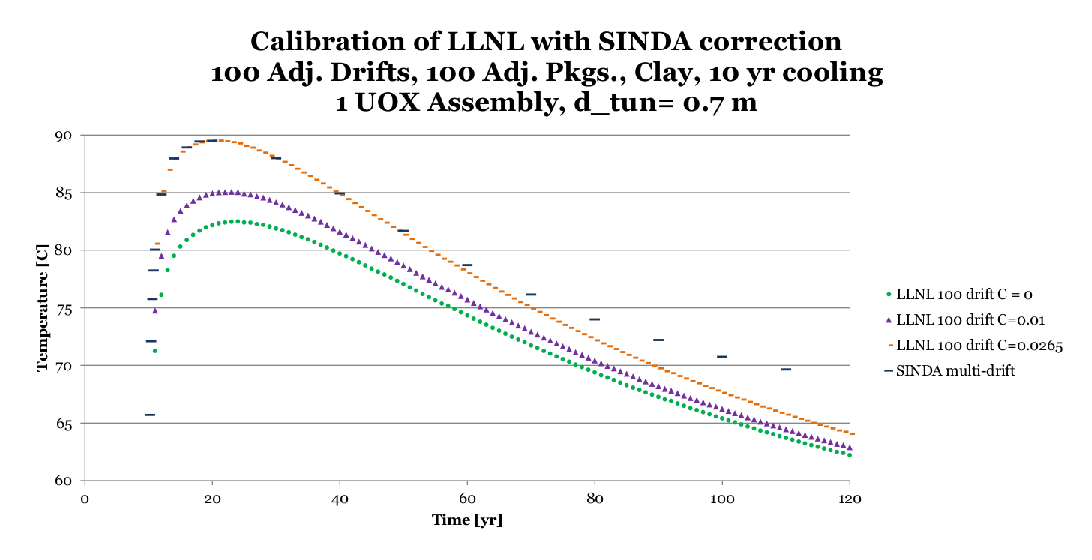
\includegraphics[width=0.5\textwidth]{100drift10yr.eps}
    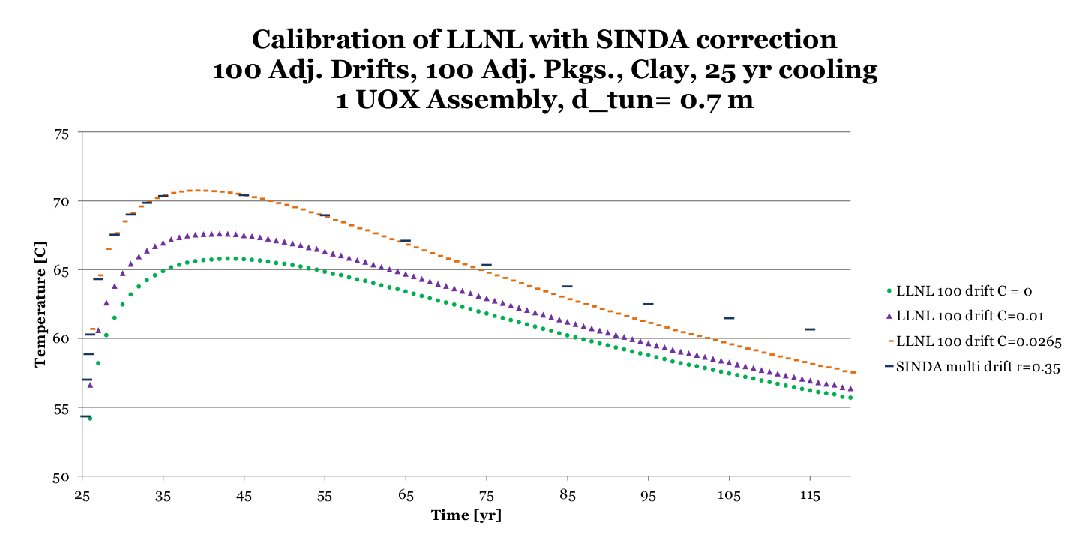
\includegraphics[width=0.5\textwidth]{100drift25yr.eps}
    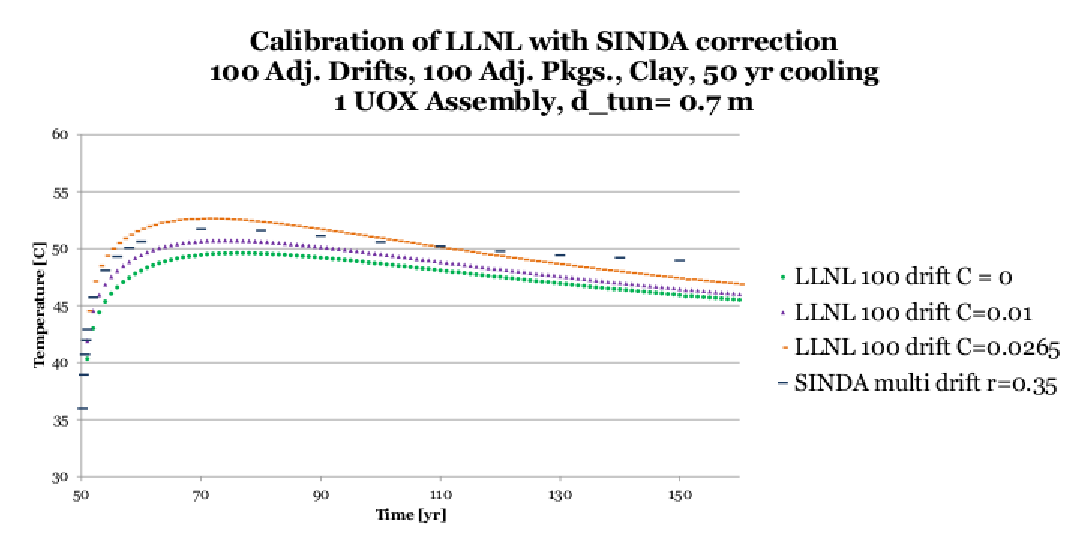
\includegraphics[width=0.5\textwidth]{100drift50yr.eps}
  \caption{A fitting coefficient of $C=0.0265m$ improves agreement for the clay 
  case with a $0.7m$ tunnel diameter and multiple drifts. The success of the fit 
  decreases for longer cooling times.}
  \label{fig:fit}
\end{figure}

For a clay repository ($K_{th} = 2.5 [W\cdot m^{-1}\cdot K^{-1}$, $\alpha = 
1.13\times10^{-6}[m^2\cdot s^{-1}$), with a tunnel diameter of $0.7m$, the 
calibration was completed using a fit between a 101 drift analytic scenario 
and the numeric model with an infinite number of drifts. $D_{d}$, the drift 
spacing, was $30m$ in each case. The results are shown in Figure \ref{fig:fit}.

%%%%%%%%%%%%%%%%%%%%%%%%%%%%%%%%%%%%%%%%%%%%%%%%%%%%%%%%%%%%%%%%%%%%%%%%%%%%%%%%
\section{Conclusions}

The result of this work is a procedure for calibration of a rapid analytic 
heat transport model which improves peak temperature value and timing agreement 
with a more detailed, but more time intensive heat transport model. With a 
single calibration, it is possible for the disagreement between the two models to 
be aleviated for many configurations. Further work toward developing a 
dimensionally appropriate theoretical dependence for the coefficient is 
forthcoming. However, we recommend that for this and other 
analytic models which neglect rapid heat transport in engineered components 
near the calculation radius, the additional step will improve results near the 
area of interest.

%%%%%%%%%%%%%%%%%%%%%%%%%%%%%%%%%%%%%%%%%%%%%%%%%%%%%%%%%%%%%%%%%%%%%%%%%%%%%%%%
%\nocite{*}
\bibliographystyle{ans}
\bibliography{ans2012}
\end{document}


